\section{Ejercicio 1: Laberinto}
    % 1. Describir detalladamente el problema a resolver dando ejemplos del mismo y sus soluciones.
    \subsection{Descripción del problema}
		    Indiana Jones continua en su expedición en la fortaleza de alguna civilización antigua. Mientras llenaban las mochilas con los tesoros que más les convenian encontraron un mapa peculiar. El mapa se parece mucho a un laberinto salvo por el hecho de que no estan conectados todos los puntos. En el mapa hay un punto que parece indicar el lugar en donde se encuentran juntando tesoros, y hay un lugar que esta indicado con una cruz. Intrigados por saber lo que se encuentra en ese lugar, se proponen como objetivo ir hacia ahi. Como nuestro equipo vino equipado con pico y pala, pueden derribar algunas paredes. Por otro lado el equipo ya se encuentra cansado y no desea recorrer mucha distancia ni esforzarse rompiendo paredes. Entonces, nos pidieron ayuda con lo siguiente: Teniendo un mapa indicando un punto de origen (identificado con una $o$) y un punto de destino (identificado con una $x$), quieren caminar lo menos posible desde el origen al destino rompiendo a lo sumo una cierta cantidad de paredes.

        La resolución del problema consiste en encontrar el camino más corto que derribe a los sumo $P$ paredes, las cuales se reconocen de un mapa dibujado con $.$ y $\#$ que indican los lugares por donde se puede pasar y las paredes respectivamente. Cada paso cuenta como 1 avance desde el origen y cuando una pared es derribada, se toma en cuenta como un lugar por el que se puede pasar, por lo que suma 1 también como parte del camino. El mapa tiene tamaño $F$ filas y $C$ columnas, los cuales se pasan por parametro al programa junto con la cantidad de paredes y el mapa. En caso de que este camino no exista, entonces la salida será solamente $-1$

        Por ejemplo, si el programa recibe lo siguiente como entrada: \newline
        \texttt{5} \texttt{9} \texttt{2} \newline
        \texttt{\# \# \# \# \# \# \# \# \#} \newline
        \texttt{\# o \# . \# . \# x \#} \newline
        \texttt{\# . \# . \# . \# . \#} \newline
        \texttt{\# . \# . \# . . . \#} \newline
        \texttt{\# \# \# \# \# \# \# \# \#} \newline

        La salida correcta sería: \newline
        \texttt{10}

    % 2. Explicar de forma clara, sencilla, estructurada y concisa, las ideas desarrolladas para la resolución del problema. Utilizar pseudocódigo y lenguaje coloquial (no código fuente). Justificar por qué el procedimiento resuelve efectivamente el problema.
    \subsection{Solución propuesta}
        Este problema resulta más simple de entender cuando se piensa el mapa como un grafo dirigido en tres dimensiones, donde la cantidad de nodos será de $FC(P+1)$ y en cada nivel habrá $FC$ nodos. De esta manera, podemos ver a cada piso del grafo (comenzando en el piso 0) como la cantidad de parades que se rompieron hasta ese punto. Los nodos estarán conectados cada uno con sus vecinos, aunque si uno de ellos es una pared, entonces el nodo se conectará con el vecino que representa a la pared pero un nivel más arriba. Hay que tener en cuenta que los nodos se modelan, para cada nivel, simplemente como el número de nodo en el grafo base (el del nivel 0) más la cantidad de nodos de cada nivel, y sus conexiónes (o aristas) se almacenan en listas de adyacencias.

        Teniendo el mapa representado de esta manera, sabemos en todo momento que la cantidad de paredes derribadas es menor o igual al límite establecido, por lo que si se puede llegar a la $x$ destruyendo una cantidad menor o igual de paredes que $P$, entonces existe un camino entre el origen y el destino.

        Para encontrar el camino mínimo entre $o$ y $x$ utilizamos el algoritmo conocido como \textit{Breadth-first Search} o \textit{BFS}, el cual conciste en recorrer el grafo analizando una sola vez cada nodo y desde éllos, observar sus vecinos. Si los vecinos de ese nodo aún no fueron analizados, se agregan a una cola para ser revisados después. Cada vez que se observa un vecino, chequeamos que no haya sido visto con anterioridad y si ese es el caso, se marca como visto cargando su distancia al origen en una \textit{lista de distancias} y agregándolo a la cola. Este algoritmo funciona en grafos donde las aristas no tienen peso o sus pesos son todos iguales, como en este ejercicio que como se dijo anteriormente, avanzar en el mapa implica sumar 1 a la cantidad de pasos, o bien aumentar en 1 la distancia al origen. Luego, los pesos de las aristas serán todos de valor 1 y puede utilizarse BFS.

        La \textit{lista de distancias} tiene el tamaño de la cantidad de nodos totales y cada posición $i$ representa al nodo $i$ del grafo. Esta lista solamente contiene la distancia al origen de cada nodo, inicializándose con $-1$ para todos y a medida que avanza el algoritmo, si el vecino $k$ del nodo $i$, que es el que se está analizando tiene distancia menor a $0$, entonces quiere decir que aún no ha sido observado.


        \subsubsection{Detalles implementativos}
            Para poder manejar correctamente el grafo, se creó la clase ListaAdy con namespace Grafos, la cual modela un grafo representado con listas de adyacencias. Las únicas operaciones que tiene la clase son el constructor, que recibe la cantidad de nodos totales, agregarArista, que recibe dos enteros $u,v$ y agrega $v$ a la lista de adyacencias de $u$, y BFS que recibe el número de nodo origen $s$, el número de origen de destino $t$, y la cantidad $f$ de filas y $c$ de columnas.
            La forma en que se almacenan las listas de adyacencias es con un vector de vectores de enteros, tipo que se provee de la librería estándar de C++.

            Normalmente, BFS solo necesitaría el nodo de origen y de destino, y almacenaría todos las posibles distancias de caminos que hay entre ambos nodos. Sin embargo, agregamos estos dos valores para que el algoritmo termine la primera vez que encuentre el nodo destino. Esto es por cómo funciona BFS: Al recorrer todos los nodos según su distancia al origen, siempre se analizan los nodos que solo están a distancia 1 más que el nodo vecino "padre" (o sea, el nodo que tenía como vecino al que se está analizando y por el cual se agregó a la cola de revisión). Ergo, si existe un camino entre $s$ y $t$, BFS encontrará el más corto antes que cualquier otro y por eso es que podemos terminar su ejecución cuando eso pase. En peor caso, no existirá un camino entre $s$ y $t$, y BFS recorrerá todos los nodos.

            El algoritmo que resuelve el problema puede separarse en dos partes: Una se encarga de leer el mapa de entrada y construir el grafo dirigido tridimensional y la otra, es el BFS que busca verdaderamente la solución.
            En la primera parte recorremos el mapa que se encuentra guardado en una matriz de \textbf{char} $P+1$ veces, para así poder construir los $p+1$ niveles del grafo y poder conectar cada nodo con sus respectivos vecinos, y para poder verificar que el mapa pasado sea válido y buscar los nodos marcados con la $o$ y la $x$.
            La segunda parte se recorre el grafo una sola vez dado el funcionamiento de \textit{BFS}, pero como tiene $FC(P+1)$ nodos, entonces esa será la cantidad de nodos que pasarán por la cola de revisión como máximo. La función BFS está implementada de la siguiente manera:


            \begin{codesnippet}
            \begin{verbatim}
BFS(enteros : s, t, f, c)
  res = -1
  cola = cola vacía
  distancias[nodosTotales]
  para i entre 0 y nodosTotales-1
    distancias[i] = -1
  fin para

  cola.encolar(s)
  distancias[s] = 0
  mientras (cola no esté vacía)
    tope = cola.tope
    cola.desencolar //al ser una cola, desencola el tope de la misma
    si (tope % (f*c)) == t
      devolver distancias[tope]
    fin si

    para i entre 0 y largo(vecinos(tope))
      si distancias[vecinos(tope)[i]] < 0
        distancias[vecinos(tope)[i]] = distancias[tope] + 1
        cola.encolar(vecinos(tope)[i])
      fin si
    fin para
  fin mientras

  devolver res
            \end{verbatim}
            \end{codesnippet}

            El único cambio que tiene esta implementación de BFS respecto de la original, es que chequea si el resultado se encuentra antes de terminar, lo cual puede hacerse por lo antes dicho. Como complemento, podemos decir que en el código puede observarse que $distancias[tope]$ siempre existe y es mayor a $0$ porque antes de agregar un nodo a la cola, se carga en $distancias$ su valor correspondiente. Además, la razón por la cual se chequea el resto de dividir $tope$ por $f*c$ es que t es el número del nodo con la $x$ en el nivel 0, mientras que al ser un grafo tridimensional donde cada nivel representa la cantidad de paredes rotas desde el origen, $t$ va a estar en todos los niveles con una diferencia de $f*c*nivelActual$. Ergo, al dividir tope por $f*c$, el resto debería ser el número de nodo que se va a analizar como si fuera uno del nivel 0.



    % 3. Deducir una cota de complejidad temporal del algoritmo propuesto y justificar por qué el algoritmo cumple la cota dada. Utilizar el modelo uniforme.
    \subsection{Complejidad teórica}

      Para este análisis, nuevamente separaremos el algoritmo en dos partes (construcción del grafo y BFS). En la primera parte, se generan $P+1$ niveles de $FC$ nodos que como se explica en el punto anterior, se representan mediante listas de adyacencias. Agregar una arista entre dos nodos cuesta $O(1)$ ya que es simplemente agregar el número de nodo destino de la arista a la lista de adyacencia del nodo origen. Hacer esto por cada nodo costaría $O(|E|)$ por cada nivel con $|E|$ siendo el número de aristas. Sin embargo, al ser un digrafo tipo \textit{grid}, la cantidad máxima de aristas por nodo es de 4 porque cada nodo se conecta con, a lo sumo, un nodo a cada lado (izquierda, derecha, arriba y abajo). Además, si bien hay $FC$ nodos en cada nivel, los nodos que sean paredes no tendrán aristas de entrada que provengan de nodos del mismo piso. Luego, $|E| \leq 4FC \in O(FC)$. Como esto ocurre $P+1$ veces, la complejidad de la primera parte es

      \[
        O((P+1)FC) \in O(FCP)
      \]


      La segunda parte, el algoritmo conocido como \textit{BFS}, tiene complejidad $O(|V| + |E|)$ siendo $|V|$ la cantidad de nodos. Ya probamos que $|E| \in O(FCP)$ y sabemos que $|V| = FC$, entonces la complejidad de la segunda parte es

      \[
        O(FC + FCP) \in O(FCP)
      \]

      Considerando las dos partes juntas, nos queda que la complejidad temporal es

      \[
        O(FCP + FCP) \in O(FCP)
      \]

      En cuanto a la complejidad espacial, el tamaño del grafo sobre listas de adyacencias es de $O(FCP)$ ya que es la cantidad de nodos totales sumado a lo que, por lo probado anteriormente, acota la cantidad de aristas totales.


    % 4. Dar un código fuente claro que implemente la solución propuesta. Se deben incluir las partes relevantes del código como apéndice del informe impreso entregado.

    % 5. Realizar una experimentación computacional para medir la performance del programa implementado. Usar un conjunto de casos de test en función de los parámetros de entrada, con instancias aleatorias e instancias particulares (de peor/mejor caso en tiempo de ejecución, por ejemplo). Presentar en forma gráfica una comparación entre los tiempos medidos y la complejidad teórica calculada y extraer conclusiones.
    \subsection{Experimentación}

	Para poder mostrar que la cota propuesta en la complejidad temporal funciona para el algoritmo que resuelve este problema, realizamos experimentos con diferentes matrices y diferentes cantidades de paredes que se pueden destruir.

  Primero se realizó un experimento con 5 matrices de tamaño 10x10. Una matriz estaba compuesta por todas paredes excepto el origen y el destino, otra tenia la mitad de paredes horizontales respecto del total de nodos, otra la mitad de paredes verticales, otra la mitad de paredes diagonales y la última no contenía ninguna pared y el origen y el destino estaban uno al lado del otro. Se optó por realizarlo de esta forma ya que se pueden probar casos límite, que son cuando se tienen que romper todas paredes, mientras que en el lado opuesto no hay que romper ninguna y el destino está a un sólo nodo de distancia del origen. Por como esta implementado el algoritmo se esperó que en los casos en donde hay que romper mucha más cantidad de paredes tarden más en ejecutarse que los que no hay que romper ninguna y además está más cerca el nodo destino del origen. Los esquemas de las matrices que se utilizaron para realizar esta parte del experimento son los siguientes:

 \begin{codesnippet}
            \begin{verbatim}
o # # # # # # # # #
# # # # # # # # # #
# # # # # # # # # #
# # # # # # # # # #
# # # # # # # # # #
# # # # # # # # # #
# # # # # # # # # #
# # # # # # # # # #
# # # # # # # # # #
# # # # # # # # # x

o # . # . # . # . #
. # . # . # . # . #
. # . # . # . # . #
. # . # . # . # . #
. # . # . # . # . #
. # . # . # . # . #
. # . # . # . # . #
. # . # . # . # . #
. # . # . # . # . #
. # . # . # . # . x

o # # # # # # # # #
. . . . . . . . . .
# # # # # # # # # #
. . . . . . . . . .
# # # # # # # # # #
. . . . . . . . . .
# # # # # # # # # #
. . . . . . . . . .
# # # # # # # # # #
. . . . . . . . . x

o # . # . # . # . #
# . # . # . # . # .
. # . # . # . # . #
# . # . # . # . # .
. # . # . # . # . #
# . # . # . # . # .
. # . # . # . # . #
# . # . # . # . # .
. # . # . # . # . #
# . # . # . # . # x

o x . . . . . . . .
. . . . . . . . . .
. . . . . . . . . .
. . . . . . . . . .
. . . . . . . . . .
. . . . . . . . . .
. . . . . . . . . .
. . . . . . . . . .
. . . . . . . . . .
. . . . . . . . . .

\end{verbatim}
            \end{codesnippet}

  El expermiento se corrío para cada matriz teniendo en cuenta que se pueden romper desde 0 hasta 99 paredes. Es decir, en total se examinaron 500 casos (100 para cada una de las cinco matrices). Además para cada caso con una determinada cantidad de paredes, se repitió el mismo experimento 100 veces para luego tomar el promedio y obtener un resultado más representativo del tiempo que tarda cada caso. Los primeros casos en los que se podían romper pocas paredes fueron los que menos tiempo de ejecución demandaron.
  Los resultados obtenidos fueron plasmados en el siguiente gráfico. El mismo es la representación del tiempo en funcion de la cantidad de paredes que se pueden romper para cada una de las cinco matrices consideredas. También se muestra la funcion propuesta como cota de complejidad temporal.

  \begin{figure}[H]
      \begin{center}
        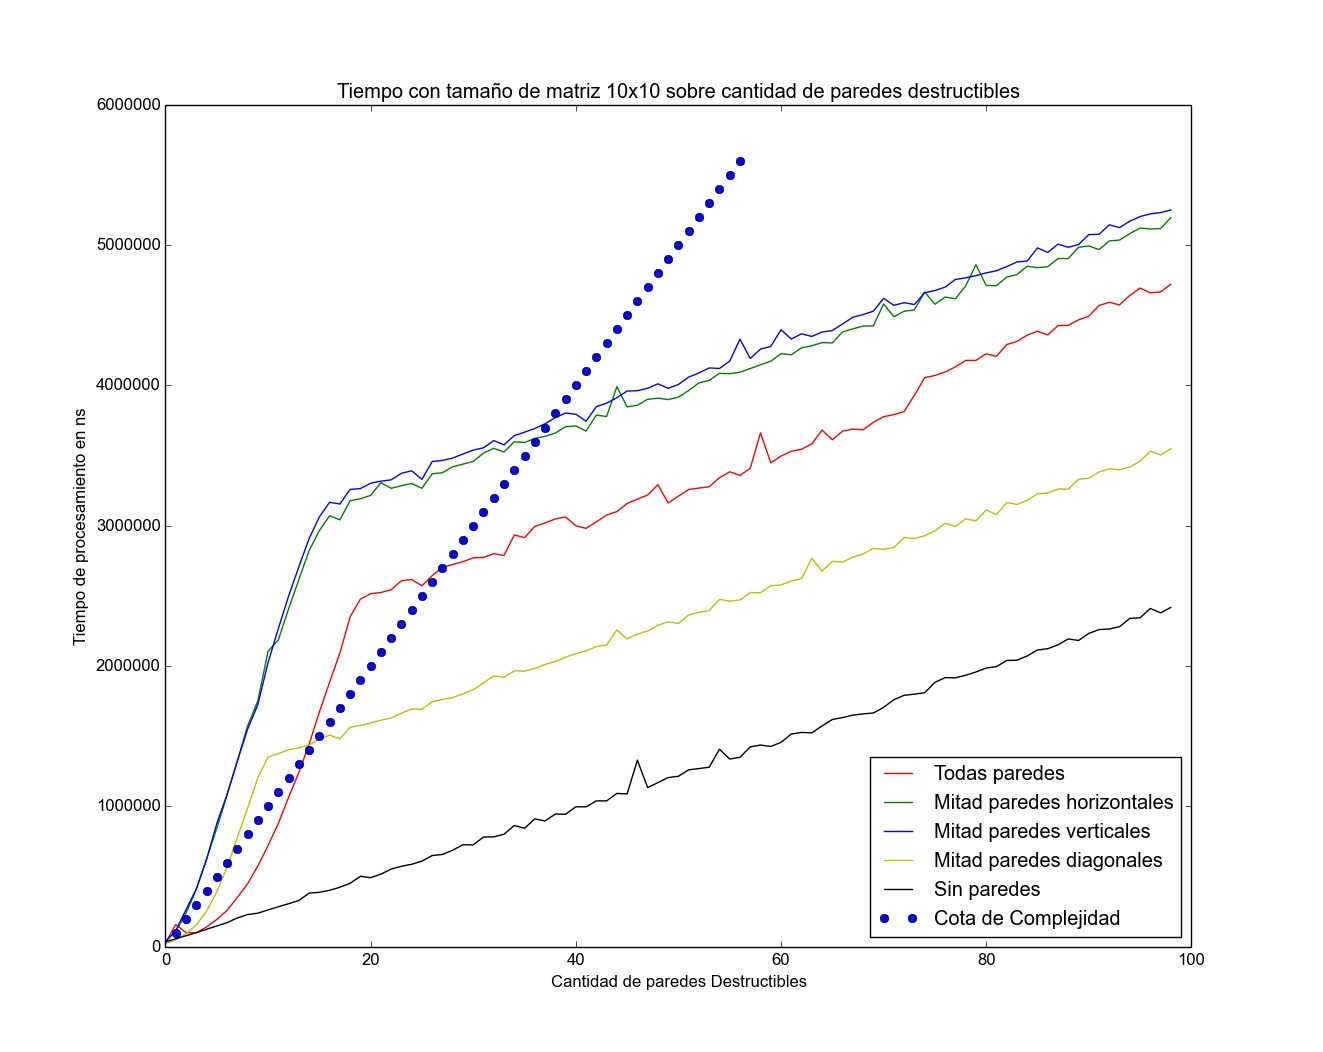
\includegraphics[width=0.7\columnwidth]{../exp/ej1tamanosFijos.jpeg}
        \caption{}
      \end{center}
  \end{figure}

  Para cada matriz puede observarse que a medida que crece la cantidad de paredes que se pueden derribar, también crece el tiempo que toma cada ejecución del programa, que era el comportamiento que se esperaba. Si bien el algoritmo de BFS corta la ejecución en cuanto encuentra el destino (en caso de poder encontrarse), no se observa una mejoría cuando se utiliza una cantidad mayor de paredes que se pueden destruir a la cantidad de nodos, debido a que en la construcción del grafo se toman en cuenta todos los niveles (cantidad de paredes), por lo que esa parte del algoritmo ya toma $O(FCP)$. Por esta razón es que el tiempo de ejecución no se mantiene constante una vez que se toma una cantidad de paredes mayor al total de nodos. El algortimo como se puede observar también tarda menos en ejecutar cuando en la matriz no hay ninguna pared y el origen y el destino están uno al lado del otro, como se esperaba. Este es el mejor caso. Los casos en los cuales había una cantidad de paredes igual a la mitad de nodos y éstas estaban en posiciones horizontales y verticales fueron aún peor que en el caso que son todas paredes. Esto puede explicarse debido a que el algoritmo de BFS inspecciona algunos vecinos que en el caso de que son todas paredes no puede ya que no tiene ningún camino que pueda pasar sin romper paredes.
  Podemos notar como la cota de complejidad cumple, aunque no de manera exacta, su función para estos experimentos.


  Luego se realizó otro tipo de experimento en el cual se utilizaron otras cinco matrices pero con tamaño y paredes dispuestas de manera aleatoria. Estas matrices fueron generadas usando la librería random de la STL con distribución uniforme. Este experimento se corrió bajo las mismas circunstancias que el otro experimento. Se corrieron 100 casos para cada una de las matrices, considerando que se pueden romper desde 0 a 99 paredes. Además también cada uno de los casos se repitió 100 veces y se tomó el promedio. Los resultados que se obtuvieron son los siguientes:

  \begin{figure}[H]
      \begin{center}
        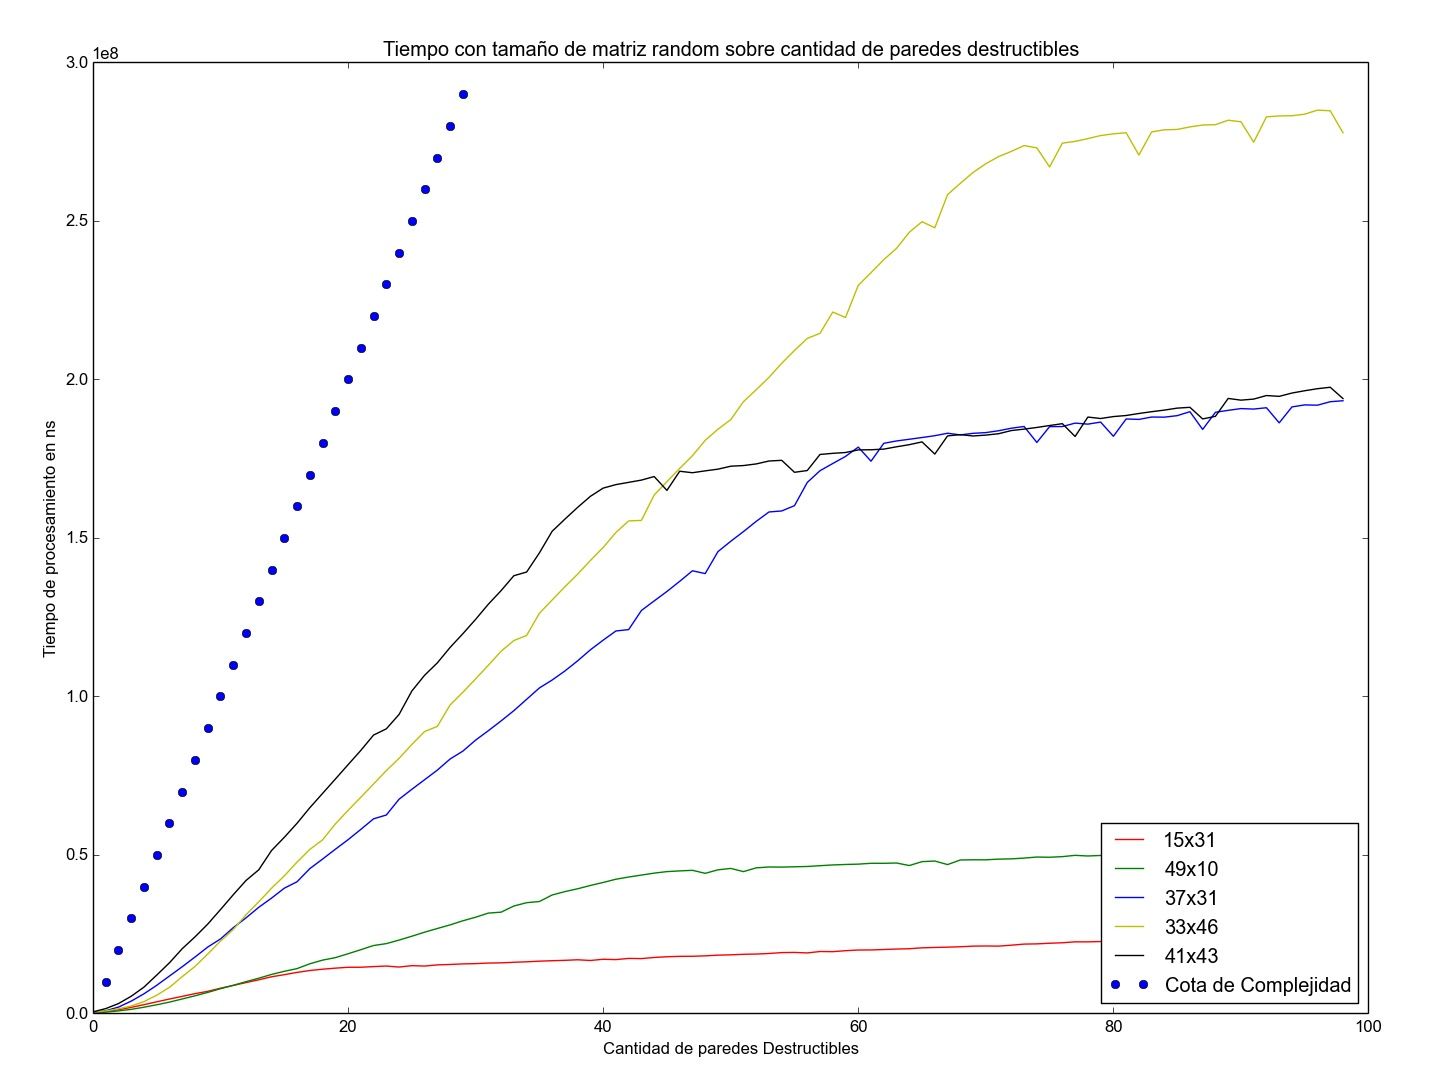
\includegraphics[width=0.7\columnwidth]{../exp/ej1tamanosRandom.jpeg}
        \caption{}
      \end{center}
  \end{figure}

  Se observa también como el tiempo de ejecución aumenta a medida de que se pueden romper más paredes para cada una de las matrices. Por lo general, los casos en los cuales la matriz tiene menos filas y columnas presentan un tiempo de ejecución menor pero pueden observarse que igualmente también depende de la cantidad de paredes que haya en la matriz. Para estos casos, la cota propuesta acota mejor de manera superior a todos los casos.
